% Copyright (c) 2014,2016 Casper Ti. Vector
% Public domain.

\chapter{PKI}

本章将对PKI系统进行详细介绍,首先从系统架构对PKI进行解析,阐述系统中包含的组成部分和各自的功能;其后将对证书进行介绍,包括证书的结构以及证书的生命周期;最后对本系统存在的问题以及相应的解决方案进行简要叙述。

\section{PKI系统}

公钥基础设施PKI(Public Key Infrastructure)作为一种遵循标准的密码管理平台,其可以为网络应用提供密钥和证书管理服务,使用户可以在多种应用环境下方便的使用加密和数字签名技术,从而保证数据的机密性、完整性、有效性和抗抵赖性。

本小节将从框架和其包含的相关组件对PKI进行介绍。

\subsection{PKI基本框架}

PKI框架中包括安全和操作策略,安全服务以及支持公钥密钥和证书管理的交互式协议。公钥和对应证书的生成、分发和管理将通过授权机构(CAs)、注册机构(RAs)和目录服务来完成\supercite{weise2001public},它们将会建立等级信任或者说信任链。以上提到CAs、RAs和目录服务可以将数字证书用于鉴定不同实体的身份,而PKI拥有如此架构的目的是为了能支持并完成数据、凭证在各种不安全环境下的安全交换。

\subsection{PKI的系统构成}

在PKI系统可能会包含一下组成部分:

\begin{itemize}
	\item 

	注册机构(RA)

	RA的作用是执行身份验证和处理新的数字证书请求、更新数字证书请求和吊销数字证书请求。

	\item

	授权机构(CA)

	CA将创建和发布数字证书以及证书吊销列表(CRLs),其颁发的数字证书将对主体名称(如用户表示)和绑定的公钥进行签名。

	\item

	验证结构(VA)

	VA是一个PKI的管理实体,可以用来检查数字证书的有效性。当证书的签发者和证书的状态管理服务有不同的服务提供者提供时,将使用到VA。

	\item

	用户

	PKI面对的用户是证书持有者或者密钥持有者,通过遵从认证运作规范(CPS)和证书策略(CP)获得证书,完成证书和密钥对的绑定。PKI系统中的用户可以是个体、组织或者非个人实体,有责任保存好自己的私钥不被泄露。

	\item

	依赖方

	依赖方在PKI系统中接收、验证和接受数字证书。

	\item

	证书策略(CP)

	证书策略是一组安全规则要求,适用于一类应用系统的共同安全需求。

	\item

	认证运作规范(CPS)

	CPS描述了CA提供数字证书服务的规则和处理方式,其中可能会包括提供服务描述,证书生命周期的管理细则、业务信息、法律义务和金融责任等。
\end{itemize}

图\ref{fig:pki}将给出以上所提到组件之间的关系,图中的剪头将表示数字证书和证书状态信息的传递。

\begin{figure}[htbp]
 	\centering
 	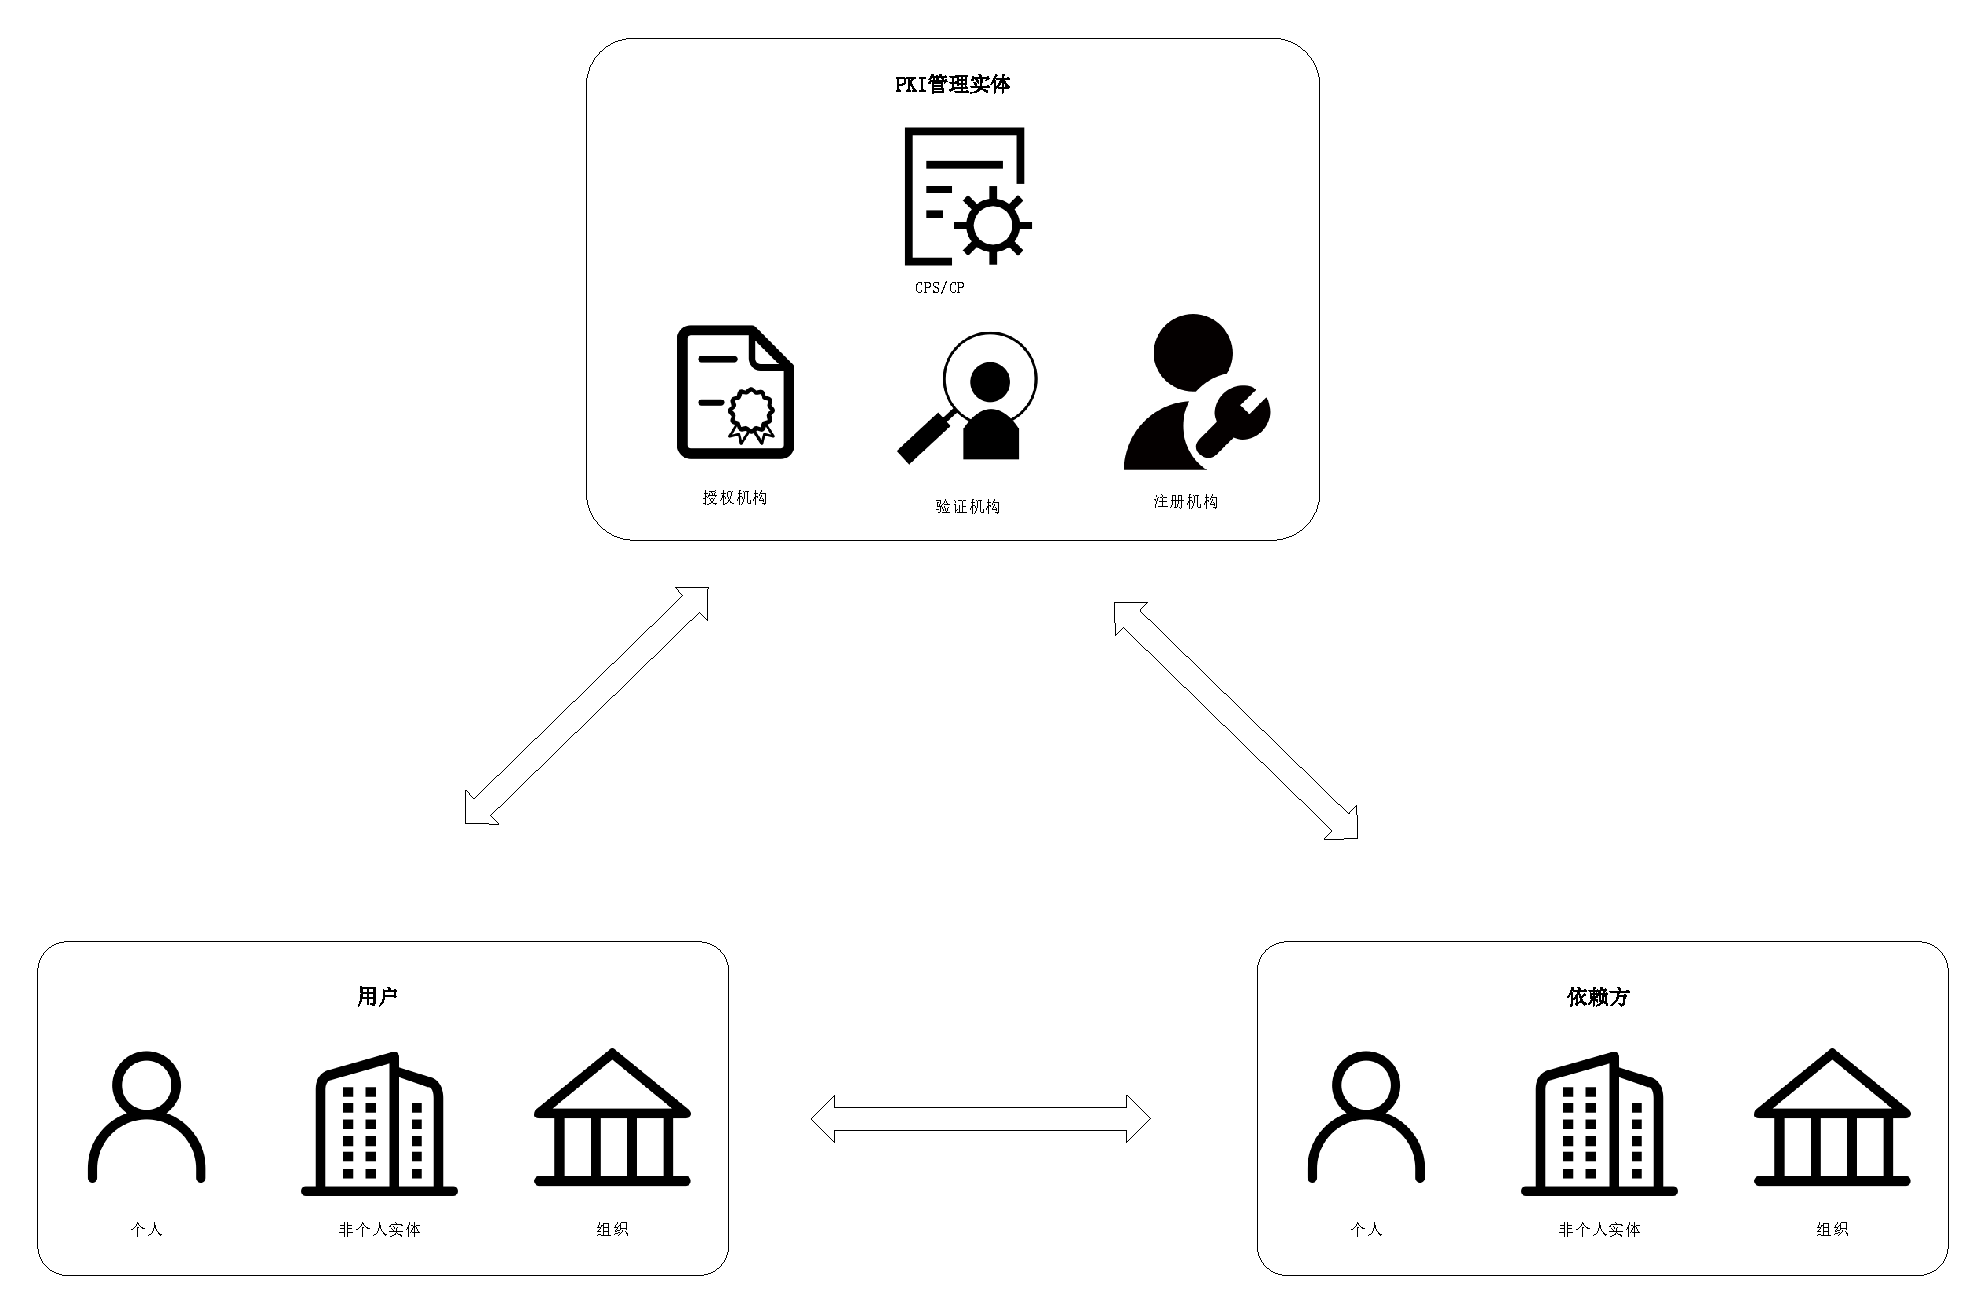
\includegraphics[width = 0.8\textwidth]{img/pki}
 	\caption{PKI组成部分}\label{fig:pki}
\end{figure}

\section{证书}

\subsection{证书的结构}

描述证书的结构。

\subsection{证书的生命周期}


证书作为包含公钥、数字签名以及一些其它附带信息的数字文档,在PKI系统中充当着公钥交换、存储和使用的介质。了解证书的申请、签发和使用,可以明白PKI系统的是如何运作,并从中发现可能存在的问题。

证书的声明周期从用户提交准备的证书签发请求(CSR)并提交给其选择的CA开始。CSR中包含了用户的公钥和相应的信息,并通过签名的方式表明对相应私钥的所有权。同时,CSR可以携带额外的信息元,但在实际使用过程中并没有全部使用。CA可以对CSR中的内容进行重写,放置一些其它的信息在证书中。

其后CA通过遵循验证流程,对用户进行身份验证。待成功完成验证之后,CA将签发证书,同时提供验证至根证书的所有中间证书。

得到证书后,用户就可在证书过期之前使用证书。如果证书对应的私钥泄露,证书将可以被吊销,该过程和证书签发的过程类似。

对于Internet PKI系统而言,根据以上证书流转流程,证书生命周期如图\ref{fig:cert_lifecycle}所示.

\begin{figure}[htbp]
 	\centering
 	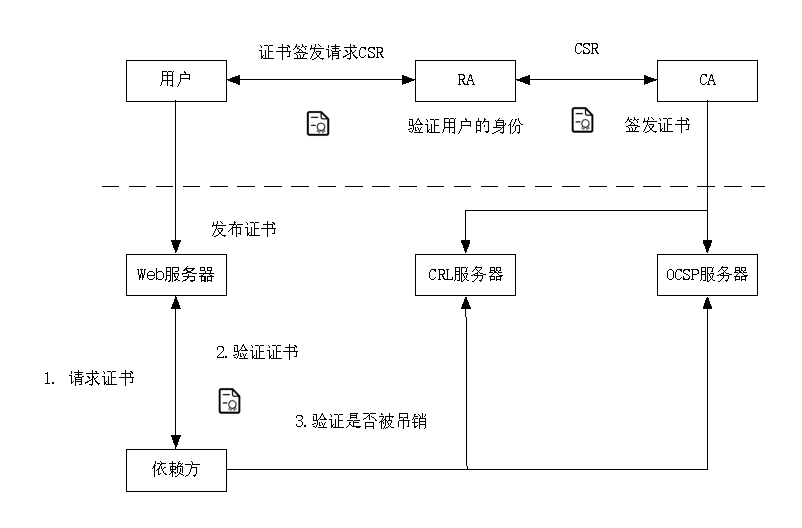
\includegraphics[width = 0.8\textwidth]{img/cert_lifecycle}
 	\caption{证书的生命周期}\label{fig:cert_lifecycle}
\end{figure}

\section{系统中存在的问题}

从安全的角度来看现有Internet PKI系统,其中存在着大大小小的各种问题,在本小节中,将对这些存在的问题进行简要概述。

当Web安全在1995年刚开始被谈及时,当时的互联网和现在是具有很大差异的,它的重要性并没有现在这么强。随着互联网的蓬勃发展,加密安全成为了商业中必备的一部分,关乎这一个企业的生死。现有的PKI系统和当初设计的目的是一致的,即为上电子商务操作提供足够的安全保障,更进一步可以说PKI系统希望提供商务安全。这种安全可以通较少的资金、更快的网页获取速度、可接受的不安全操作和不对用户做过多的限制来完成。本系统由CAs、寻利的商业实体和希望扩大市场份额的游览器供应商一起来组成。

CA在本系统中充当着信任的基础,其每年签发了数百万计的证书,这些证书将在互联网中流通并使用。虽然证书的安全性并没有想象中那么好,但是这个系统任然在正常的运转下去。同时,在那么不完美的情况下,用户还需要对申请的证书进行付费,然而并不是所有用户都愿意为之付出代价的,很简单的一个原因就是他们在付费之后希望得到完美的安全性保障。

在该系统中,存在着一下几个方面的问题:


\begin{itemize}
	\item

	域名权利过弱

	在PKI系统中最大的问题是任意CA在未经域名同意的情况下就可以对其签发证书,导致这个问题的主要原因是没有相关的技术策略去避免CA的疏漏和安全隐患,而该系统需要对CA给予相当高的信任。当CA数量比较少的时候,这个问题并没有那么严重,但是下周乃有数以百计的CA存在,很难保证每一个都不会存在行为过失或者不当的安全配置。一个系统的安全性取决于该系统最薄弱的环节,而PKI系统中存在着各种潜在的薄弱环节。所有的CA都需要被审计,但是审计的质量缺是不确定的。例如在2011年DigiNotar由于自身安全性问题就被黑客攻陷,最后导致自身倒闭。

	同时,另外一个存在的问题是CA是否可以被信任,它们能否在不需要监督的情况下为了公众的利益去做好自己的本质工作。这些被信任的CA可能在面对商业利益的时候放弃我们需要的安全。例如在2012年Trustwave承认其签发了低级别的假冒证书用于流量检查。虽然Trustwave是唯一公开承认自己做过类似事情的CA,大家相信这样的事情肯定大量存在。

	政府也可能会滥用PKI系统签发虚假证书,完成对任意域名的假冒。公众无法确保CA不会作为证书的前线,即使不是也无法保证这些CA不会被强迫的签发虚假证书。



	\item

	没有信任灵活度

	另外一个重要的问题是本系统缺乏信任的灵活度。依赖方将会存储一些列信任的根证书,一个CA只存在信任与否,并不存在中间地带。理论上,依赖方可以移除任何存储的CA,实际上这种情况只会在CA很小或者其已经被攻陷的时候发生。一旦一个CA签发了大量的证书,其将由于自身的大体量被不会被撤销。

	一些小的改善任然在被提出,例如对具有过失行为的CA不在信任打,是其之前的证书任然可以被使用。

	\item

	域名验证过于简单

	DV证书的签发是基于域名的WHOIS协议查询域名拥有者信息来完成的,也就是说大部分验证是通过邮件来完成的,而其本身的安全性就存在问题。如果域名被黑掉或者相应的邮箱密码被获取,那么就可以得到给域名的DV证书。同时通过拦截CA端验证信息也可以对发起攻击。



	\item 

	吊销不工作

	在一般情况下,对吊销证书的检查并没有那么严格,大多数情况都不能正常的工作。在2011年中有很多这样的例子,依赖方不得不将被泄露的证书通过特殊通信方式下载并存储在黑名单中,来保证吊销查询是可靠的。

	这样做的原因主要包括两个,首先将吊销信息发送各个系统需要一定的延时,在基准规则中允许CRL和OCSP的信息在10天是有效的,也就是说至少需要10天才能保证吊销信息被完全扩散出去;其次软失败机制在所有的游览器中被使用,当他们在查询吊销信息时会忽略掉所有失败的情况,一个主动的网络攻击者将可以轻易的拦截OCSP的请求,保证他们使用虚假的证书可以完美的被使用。

	由于以上的原因,Chrome开发者取消去证书吊销的检查,除非是EV类型的证书。对于重要的证书,例如中间证书,其间依赖于CRL信息的吊销通道查询相关内容。一种可能的解决方案是使用Must-stale的方案来保证证书的有效性。

\end{itemize}


\section{已有的改善措施}

为了解决X.509 PKI中的安全问题并削弱对CAs的信任,一系列的方案被提出来,本小节将对这些方案进行分类并简要叙述。



根据PKI中存在的主要三方实体域名、CA和客户端,可以对现有的方案进行分类,如图\ref{fig:Classification_of_PKI_proposals}所示。

\begin{figure}[htbp]
 	\centering
 	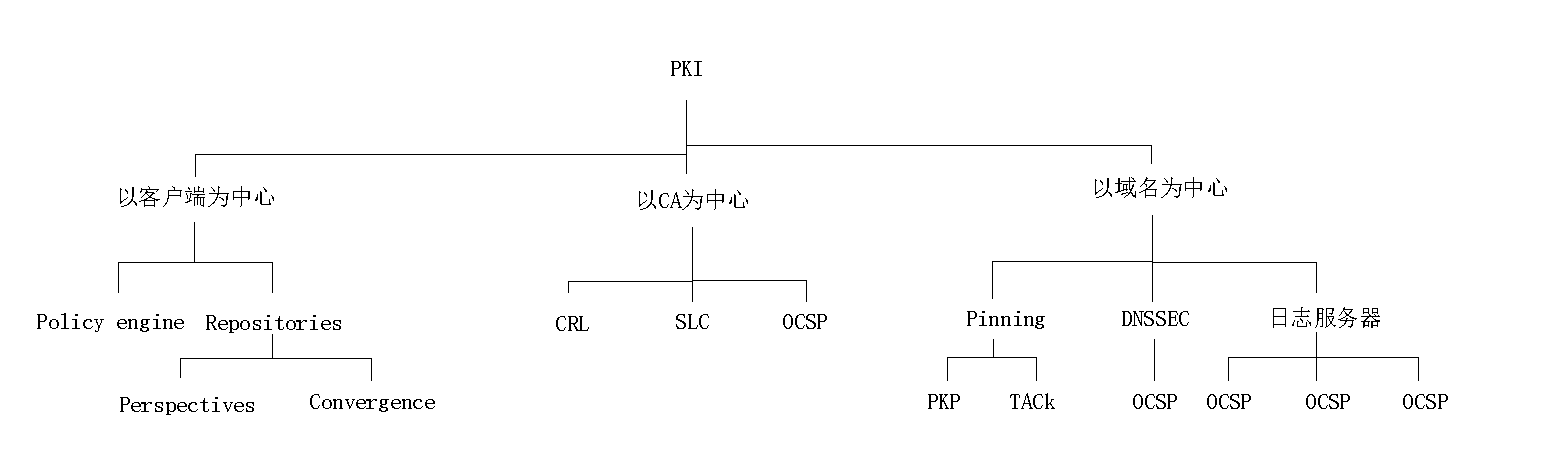
\includegraphics[width = 1.0\textwidth]{img/Classification_of_PKI_proposals}
 	\caption{PKI方案分类}\label{fig:Classification_of_PKI_proposals}
\end{figure}



\subsubsection{以客户端为中心的方案}

这类方案希望在客户端接受证书之前,可以更加准确的验证证书的有效性。Policy engine的方案允许客户端在本地制定信任决策,比如支持的密码算法,证书的一致性性等。

有一些其它的方案希望构建一个公共的域名证书存储厂库,使得客户端可以在接受到域名证书之后与厂库中的证书进行对比,确定证书的正确性,Perspectives 和 Convergence就输入这类方案。

以客户端为中心的方案并不需要对服务端进行的改动,但是其需要客户端建立额外的连接去查询资源厂库,这将在一定程度上降低建立HTTPS的速度。


\subsubsection{以CA为中心的方案}

X.509 PKI包含了证书吊销列表(CRL)标准,希望放置客户端与一个使用已经被吊销证书的域名之间发起建立TLS连接。但是这需要保证客户端需要能随时的访问到CRLs。为了进一步解决在线验证的问题,在线证书状态协议(OCSP)允许客户端通过CA的OCSP服务器去检查域名证书的状态。但是OCSP也拥有如安全、隐私、性能方案的顾虑。另外一个解决方案是短期证书(SLC),该方案希望签发短声明周期的证书,让域名定期的更换证书。SLC希望提带来和OCSP类似的好处,但是不需要在线验证。以证书为中心的方案严重依赖于游览器去检测和拉黑被攻陷CA签发的证书,这是这类方案的最大缺陷。


\subsubsection{以域名为中心的方案}


第三类方案允许域名拥有者积极控制和保护他们的证书而不被CA端的潜在问题所威胁。这些方案又可以分为以下三类:pining、DNSSEC、日志服务器。

1. Pinning-based(公钥固定)

如Public Key Pining(PKP)和Trust Assertions for Certificate Keys(TACK)等Pinning的方案希望域名宣称自己使用的密钥,以便客户端收到的密钥是否正确。但是这类方法有相应的安全缺陷,比如在第一次访问域名的时候无法给予安全保护。

2. DNSSEC-based

这类方案的全称叫基于DNS的命名实体鉴权(DANE),希望域名的所有者可以在DNSSEC实体上方式证书相关的特殊声明,例如可以为其签发证书的CA名单、声明接受的证书或者是声明验证证书有效性的节点,但是DANE的安全性严重的依赖于DNS操作的安全性行。


3. 日志服务器

另外一种使用比较多的方法是通过日志服务器的方案来记录CA的行为,为域名拥有者提供公共的、可审计的CA行为日志,监督CA的行为。例如 Sovereign Keys (SK)要求域名拥有者生成一个主密钥对来完成对TLS公钥的签名,并且将其主公钥以只读和只可追加的方式记录在时间服务器上。不行的是,SK需要客户端查询服务器,增加了延迟并牺牲了隐私。

证书透明(CT)的方案允许每个域名将自己的证书注册记录到一个公共日志服务器上,该服务器使用默克尔哈希树的结构来存储这些证书,并保证只能追加的性质。该服务器将返回一个不可否认的证书审计证明给域名,域名使用证书和该证明给客户端来完成TLS连接的建立。但是,本方案并不能防止当一个攻击者攻破了CA并创建并注册一个虚假的证书的情况,CT并不能阻止客户端接受这类证书。由于证书透明在设计过程中并没有强调证书的吊销,相应的证书吊销透明(RT)也被提出。为了提高CT对证书吊销的效率,证书签发吊销透明(CIRT)方案被提出。

另外一种基于日志服务器的方案称作可审计密钥设施(AKI),该方案希望保护域名和客户端遭受到单点失败攻击,比如某个CA的根密钥被泄露,通过制衡该系统中各个实体,AKI在保持高效处理证书操作的情况下,成功的将信任分散到了多个实体,并可以检测出实体的恶意行为。




% vim:ts=4:sw=4

























































